%% Author_tex.tex
%% V1.0
%% 2012/13/12
%% developed by Techset
%%
%% This file describes the coding for rsproca.cls

\documentclass[openacc]{rsproca_new}%%%%where rsproca is the template name


\usepackage{graphicx}
\usepackage{amsmath}
\usepackage{amssymb}
\usepackage{bm}

\newcommand{\ie}{i.\,e.~}
\newcommand{\Ie}{I.\,e.~}
\newcommand{\eg}{e.\,g.~}
\newcommand{\Eg}{E.\,g.~}
% \newcommand{\e}{\mathrm{e}}
\newcommand{\ic}{i}

\newcommand*\conj[1]{
  \vbox{
  \hrule height 0.3ptword
  \kern0.5ex
  \hbox{
  \kern-0.4em
  \ifmmode#1\else\ensuremath{#1}\fi
   \kern-0.em
  }
 }
}
\newcommand{\B}{\boldsymbol}
% \newcommand{\tens}[1]{\B{#1}}
% \newcommand{\tens}[1]{\underline{\underline{#1}}}
\newcommand{\tens}[1]{\B{#1}}
\newcommand{\re}{\mathrm{Re}}
\newcommand{\im}{\mathrm{Im}}
\newcommand{\grad}{\B{\mathrm{\nabla}}}
\renewcommand{\div}{\B{\mathrm{\nabla\cdotp}}}
\newcommand{\ddroit}{\mathrm{d}}
\newcommand{\epsf}{\varepsilon^{\rm f}}
\newcommand{\epsftens}{\tens{\varepsilon}^{\rm f}}
\newcommand{\epstens}{\tens{\varepsilon}}
\newcommand{\epsd}{\varepsilon^{\rm d}}
\newcommand{\epsvac}{\varepsilon_{0}}
\newcommand{\epshom}{\tilde{\epstens}}
\newcommand{\fig}[1]{Fig.~(\ref{#1})}
\newcommand{\equ}[1]{Eq.~(\ref{#1})}

\newcommand{\xitens}{\tens{\xi}}
\newcommand{\xihom}{\tilde{\xitens}}


%%%% *** Do not adjust lengths that control margins, column widths, etc. ***

%%%%%%%%%%% Defining Enunciations  %%%%%%%%%%%
\newtheorem{theorem}{\bf Theorem}[section]
\newtheorem{condition}{\bf Condition}[section]
\newtheorem{corollary}{\bf Corollary}[section]
%%%%%%%%%%%%%%%%%%%%%%%%%%%%%%%%%%%%%%%%%%%%%%%


\begin{document}

%%%% Article title to be placed here
\title{Homogenization of periodic and random ferroelectric-dielectric composites}
\author{Benjamin Vial and Yang Hao}

%%%%%%%%% Insert author address here
\address{School of Engineering and Computer Science, Queen Mary, University of London, London, E1 4NS, United Kingdom}

%%%% Subject entries to be placed here %%%%
\subject{xxxxx, xxxxx, xxxx}

%%%% Keyword entries to be placed here %%%%
\keywords{Homogenization, Ferroelectrics, Metamaterials , Tunability}

%%%% Insert corresponding author and its email address}
\corres{Benjamin Vial\\
\email{b.vial@qmul.ac.uk}}

%%%% Abstract text to be placed here %%%%%%%%%%%%
\begin{abstract}
  We investigate the homogenized permittivity of ferroelectric-dielectric mixtures under
  a static electric field. A refined model is used to take into account the coupling
  between the electrostatic problem and the electric field dependent permittivity of the
  ferroelectric material. Periodic and random structures in two dimensions are investigated and
  we study the effective permittivity, losses, electrically induced anisotropy and tunability
   of those metamaterials.
\end{abstract}
%%%%%%%%%%%%%%%%%%%%%%%%%%%

%%%%%%%%%% Insert the texts which can accomdate on firstpage in the tag "fmtext" %%%%%

\begin{fmtext}
  \section{Introduction}
  Ferroelectric materials play a crucial role in reconfigurable 
  microwave devices, with typical applications including antenna beam steering,
  phase shifters, tunable power splitters, filters, voltage controlled oscillators and
  matching networks \cite{tagantsev_ferroelectric_2018}. Both bulk ceramics and thin films have
  been employed to design frequency agile components \cite{vendik_ferroelectric_1999, lancaster_thin-film_1998,xi_oxide_2000} and metamaterials \cite{hand_frequency_2008, zhao_experimental_2008}. The main reason of using
  ferroelectric materials is their strong dependence of their permittivity $\varepsilon$
  on an applied electric field $E$, which is measured by their tunability defined as $n = \varepsilon(0)/\varepsilon(E)$.
  The key requirements for antenna and microwave applications are large tunability and low losses.
  These two characteristics are correlated and one has to find a trade-off for optimal device
  performance, which can be quantified by the so called commutation quality factor
  $K = (n -1)^2/(n\, \tan\delta(0)\,\tan\delta(E))$, where $\tan\delta$ is the loss tangent.\\
  These materials have usually high permittivity values,
  often leading to slow response time and impedance mismatch, which can be an issue in some practical
  applications. Thus it has been considered to mix ferroelectric ceramics to low-index and
  low-loss non-tunable dielectrics in order to reduce both permittivity
\end{fmtext}

%%%%%%%%%%%%%%% End of first page %%%%%%%%%%%%%%%%%%%%%

\maketitle
\noindent values and losses.
The effective parameters of those composites have been investigated \cite{sherman_ferroelectric-dielectric_2006, jylha_tunability_2008, sherman_tunability_2004, astafiev_can_2003} and it has been found that the
permittivity can be greatly reduced while losses and tunability are much less sensitive to the
dielectric phase addition.\\
This study investigates the effective permittivity of dielectric/ferroelectric composites
by using a two-scale convergence method \cite{allaire_homogenization_1992, guenneau_homogenization_2000}.
The originality lies in the fact that a fully coupling model is employed to
calculate the electrostatic field distribution when a uniform biasing field is
applied on the structures, which will result in a local modification of the permittivity
in the ferroelectric phase due to the microstructure. As compared to a simple uncoupled model where the
ferroelectric phase is only modified through the biasing field,
the resulting effective permittivity, dielectric losses, tunability and
anisotropy significantly differ. \\
We study first a two-dimensional model of metamaterials made of parallel rods with circular cross section,
considering both square periodic arrays and random distributions within the unit cell of
a periodic array.


%#########################################################################################

\section{Theory and numerical model}

We consider a composite made of a ferroelectric material with anisotropic
permittivity $\epsftens(\B E)$
that is dependent on an applied electric field $\B E$,
and a non tunable dielectric of permittivity $\epsd$, which are both non-magnetic.
The structures under study are invariant along the $z$ direction, which leads to the standard decomposition
of the wave equation in the transverse electric case (TE, electric field parallel
 to the direction of invariance) and the
transverse magnetic case (TM, magnetic field parallel to the direction
of invariance).
A uniform biasing field is applied to the sample in order to be able to tune the
permittivity of the dielectric phase.
Modelling homogenized properties of this type of mixtures can be done by assuming
that the electric field distribution is uniform throughout the sample,
so that the study of the tunability is
essentially achieved by changing the value of the properties in the ferroelectric phase and computing
 the effective permittivity
of the composite. We refer this approach as to the uncoupled model in the following.
However, a more accurate description is to take into account the change of the
electric field by the microstructure, if any. We therefore need to solve an
electrostatic equation to find the field distribution within the material, but its solution
depends on the permittivities of both materials, and the permittivity in the
ferroelectric phase depends on this induced electric field: this leads to a strongly coupled problem.\\

% -------------------------------------------------------------------------------
\subsection{Permittivity model\label{permmodel}}

We use barium strontium titanate (BST) as our ferroelectric material. Measurements
have been carried out at electrostatics and at microwave frequencies, and the normalized permittivity value
as a function of biasing field are reported on \fig{fig1}.\\
To describe the permittivity, we make use of the Landau potential
given by $F(P,E) = F_0 +  a P^2/2 + b P^4/4 + cP^6/6 - EP$, where $E$ is
the applied electric field and $P$ is the polarization \cite{landau_electrodynamics_2013, zhou_dielectric_2008}. Variations of the
permittivity with the temperature can be taken into account through the
 coefficients $a$, $b$ and $c$, but we assume we are working at a constant
room temperature. We further assume that the material is not subject to any stress, so that the variation
of permittivity due to mechanical constraints is irrelevant.
The equation of state $$\frac{\partial F (P, E)}{\partial P}   = a P_0 + b P_0^3 + c P_0^5 - E = 0$$ gives the
dependence of the polarization on the applied electric field,
with $P_0$ being the equilibrium polarization.
Along the direction of a uniform applied electric field, the relative permittivity is given by:
\begin{equation}
  \epsf(E) = \left[\frac{\partial^2 F (P, E)}{\partial P^2} \right]^{-1} = \frac{\epsf(0)}{1 + \alpha P_0^2 + \beta P_0^4},
  \label{eq_epsf}
\end{equation}
where $\epsf(0)=1/a$, $\alpha=3b/a$ and $\beta=5c/a$. The fitting parameters are given in Table \ref{table_params_fit}.
As the norm of the field increases, the permittivity decreases with a characteristic
bell curve typical for a ferroelectric material in its paraelectric state.
\begin{figure}[!t]
\centering
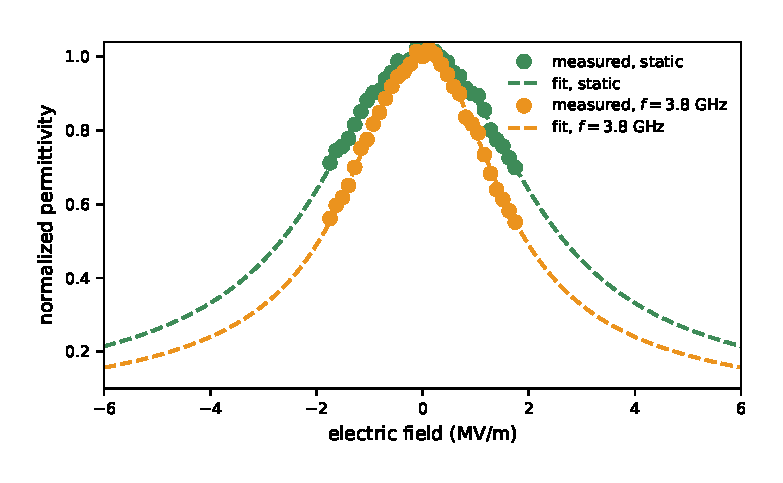
\includegraphics[width=0.8\columnwidth]{epsilon_fit}
\caption{Variation of the ferroelectric permittivity as a function of the
 applied electric field (dots: measurements, dashed lines: fit to
 formula~(\ref{eq_epsf})), for the static case (green) and at microwave frequencies
  (orange, $f=3.8$ GHz). The fitting parameters are given in Table \ref{table_params_fit}.}
\label{fig1}
\end{figure}
Furthermore, assuming the crystalline principal axes of the ferroelectric material
are oriented in the coordinate directions, and that the diagonal components of the permittivity
tensor are only function of the corresponding bias electric field components \cite{krowne_anisotropic_2002}, we have:
\begin{equation}
  \epsftens (\B E) =
\left(
\begin{matrix}
\epsf_{xx}(E_x) & 0 & 0 \cr
0 & \epsf_{yy}(E_y) & 0 \cr
0 & 0 & \epsf_{zz}(E_z) \cr

  \end{matrix}
  \right)
\label{eq_epsftens}
\end{equation}
where each of the diagonal components have the functional form
given by \equ{eq_epsf}. Note that we will use the static values of permittivity
for the electrostatic modelling, while we are interrested in the homogenized values
of permittivity at microwaves.\\
\begin{table}
  \caption{Fitting parameters to model (\ref{eq_epsf}) for the measured permittivity values as a function
  of applied electrc field shown on \fig{fig1}. }
  \label{table_params_fit}
  \begin{tabular}{llll}
    \hline
   case & $\epsf(0)$  & $\alpha$ ($\rm \mu m^2/V^2$) & $\beta$ ($\rm \mu m^4/V^4$)\\ \hline
  static & 3050 & 0.120 & 0.024\\
  $f=3.8$ GHz & 165 & 0.240 & 0.079 \\\hline
  \end{tabular}
\end{table}


% -------------------------------------------------------------------------------
\subsection{Electrostatic model}
The composites under study are made of two materials, thus their permittivity
is represented by a piecewise defined tensor $\epstens(\B r, \B E)$ which is
equal to $\epsftens(\B E(\B r))$ in the ferroelectric phase and ${\rm diag}(\epsd)$
in the dielectric phase.
In the following, we consider two different cases for the biasing field.
Because of the form~(\ref{eq_epsftens}) assumed for the ferroelectric permittivity
tensor, $\varepsilon_{zz}$ will not be changing for a field in the plane orthogonal
to the $z$ axis. This is the only component
being relevant for TE polarization, so we consider in this case a uniform biasing
electric field applied along the direction of invariance $\B E_0 = E_{0} \B e_z$.
On the other hand,
the in-plane components of $\epsftens$ are tuned by $E_x$ and $E_y$, therefore,
without loss of generality,
we consider a uniform applied electric field directed along the $x$ axis
$\B E_0 = E_{0} \B e_x$ for the TM polarization case.
To calculate the total electric field in the material, one
has to solve the electrostatic equation for the potential $V$:
\begin{equation}
\div (\epsvac \epstens \grad V) = 0
\label{eq_elstat}
\end{equation}
Note that for the TE case, the solution is trivial since the structures
are invariant along $z$, so that the electric field is equal to the uniform biasing field, and
we will therefore not study it in the following.
However in the TM case, the situation is much more complex: this is a coupled problem since the
electric field $E=-\grad V$ derived from the
solution of \equ{eq_elstat} depends on the permittivity distribution, which
itself depends on the electric field.
The coupled system formed
of Eqs.~(\ref{eq_epsftens}) and (\ref{eq_elstat}) is solved iteratively until there
is convergence on the norm of the electric field.
Here we would like to emphasise that the permittivity in the ferroelectric material, although
uniform initially, will be spatially varying due to the non-uniform distribution
of the total electric field.\\

% -------------------------------------------------------------------------------
\subsection{Homogenization}
The effective permittivity for TM polarization is calculated
using two scale homogenization technique \cite{allaire_homogenization_1992, guenneau_homogenization_2000}.
For this purpose, one has to find the solutions
$\psi_j$ of two annex problems $\mathcal P_j$, $j=\{1, 2\}$:
\begin{equation}
\div \left[ \xitens \grad(\psi_j + r_j) \right] = 0,
\label{eq_hom_annex}
\end{equation}
where $\B r = (x, y)^{\rm T}$ is the position vector in the $xy$ plane and
$\xitens=\epstens^{\rm T}/ {\rm det }(\epstens)$.
The homogenized coefficient $\xihom$ is obtained with:
\begin{equation}
\xihom = \langle \xitens \rangle + \B \phi,
\label{eq_hom}
\end{equation}
where $\langle . \rangle$ denotes the mean value over the unit cell.
The elements of the matrix $\B \phi$ represent correction terms and
are given by $\B \phi_{ij} = \langle \xitens \grad \psi_i \rangle_j$.
Finally the homogenized permittivity  can be calculated using $\epshom=\xihom^{\rm T}/ {\rm det }(\xihom)$.\\
Note that the TE case, which we shall not study here as no coupling happens, is trivial since
the homogenized permittivity is simply the average of the permittivity in the unit cell:
$\epshom = \langle \epstens \rangle$.


% -------------------------------------------------------------------------------
\subsection{Numerical setup}
Equations~(\ref{eq_elstat}) and (\ref{eq_hom_annex}) are solved with a Finite Element
Method using the open source packages Gmsh \cite{geuzaine_gmsh:_2009} and GetDP \cite{dular_general_1998}.
In both cases we use a square unit cell $\Omega$ of length $d$ with periodic boundary
conditions along $x$ and $y$. Second order Lagrange elements are used and the
solution is computed with a direct solver (MUMPS \cite{amestoy_fully_2001}).
% The source code and
% data necessary to reproduce the results reported in this paper are freely available
% online.


%#########################################################################################

\section{Numerical results}
In the following numerical results, the dielectric phase is supposed to be
lossless and non dispersive with $\epsd = 3$ while the ferroelectric material follows the
permittivity described in section~\ref{permmodel} and has a constant loss
tangent $\tan \delta^{\rm f} = 10^{-2}$.



% -------------------------------------------------------------------------------
\subsection{Two dimensional periodic metamaterial}
\begin{figure}[!t]
\centering
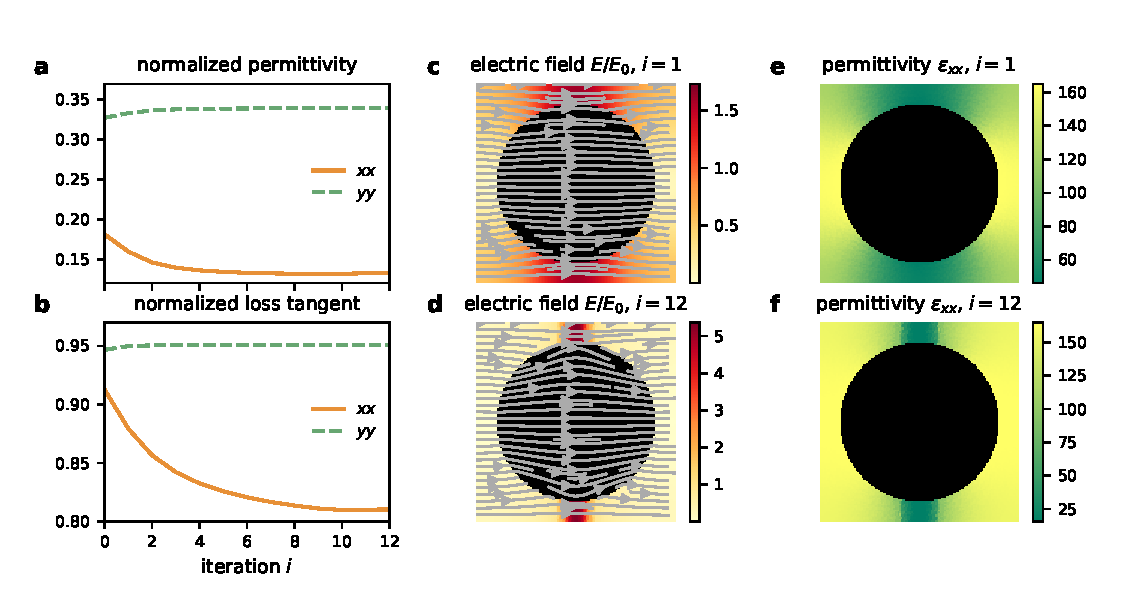
\includegraphics[width=1\textwidth]{conv_per}
\caption{Convergence of the coupled problem.
Real part (a) and loss tangent (b) of the components of the homogenized
 permittivity tensor as a function of iteration step $i$. The distribution of
 the normalized electric field (colormap: magnitude, arrows: direction) and of the
 $xx$ component of the permittivity tensor are shown for $i=1$
  (c and d) and $i=12$ (e and f).
 }
\label{conv2D}
\end{figure}
Lets us now consider infinitely long dielectric rods of circular cross section
of radius $r$ embedded in a ferroelectric matrix.\\
We first study the convergence of the coupled problem on the particular case with dielectric
filling fraction $f=\pi r^2/d^2=0.5$ and $E_0=2$kV/mm. Figures \ref{conv2D}(a) and \ref{conv2D}(b) show the
convergence of the real part and loss tangent of the components of the homogenized
 permittivity tensor, respectively. The $yy$ components converge very quickly
 and are almost unaffected by the coupling process whereas the
 $xx$ components change substantially from the initial conditions.
 This is due to the effect of the distribution
 of the electrostatic field within the unit cell (see Figs.~(\ref{conv2D}.c) and (\ref{conv2D}.d)),
 where the $x$ component of the electric field is still much stronger
 than the $y$ component, even if it is spatially varying in the ferroelectric medium.
 At equilibrium, the electric field is concentrated close to the $y$ axis in between two neighbouring
 rods. This in turn affects the permittivity distribution (see Figs.~(\ref{conv2D}.e) and (\ref{conv2D}.f)),
 and the homogenized properties of the composite.\\
 We computed the effective parameters of these metamaterial structures for different
 radii of the rods and studied their behaviour when subjected to an external
 electrostatic field (see \fig{eff_par_2D_TM}). The results of our coupled
 model differ significantly from the uncoupled one. Increasing the dielectric fraction
 lowers the effective permittivity while the losses are slightly reduced but much less sensitive.
 Due to the inhomogeneous redistribution of the permittivity over the ferroelectric domain, the
 overall tunability changes. In the case studied here, taking into account the coupling leads to an effective tunability increase with
 higher dielectric concentration, and that is larger than the tunability of bulk ferroelectric.  There are two concurrent effect at stake here: on the one hand
 the dilution of ferroelectric makes the composite less tunable, but on the other hand,
 the rearrangement of the electrostatic field surrounding the inclusion and its
 concentration in some region will cause a higher permittivity change locally.
 The relative strength of those phenomena is governed by the shape of the inclusion and its permittivity
 and so it is envisioned that the performance of the composites might be enhanced by engineering
 their microstructure.
 The geometry of the unit cell is symmetric so the homogenized material is
  isotropic when no field is applied.
 But when the sample is biased, the permittivity distribution becomes asymmetric due
 to the inhomogeneity of the electric field, thus making the effective material properties anisotropic.
This geometric effect is added to the anisotropy arising from the material properties of the ferroelectric
phase itself, and depending on the topology and permittivity of the rods, one effect would be predominant.
Those subtle phenomena can only be rigorously taken into account by employing a coupling formalism
and are responsible for the difference observed when compared to a simple uncoupled model.\\



\begin{figure}[!t]
\centering
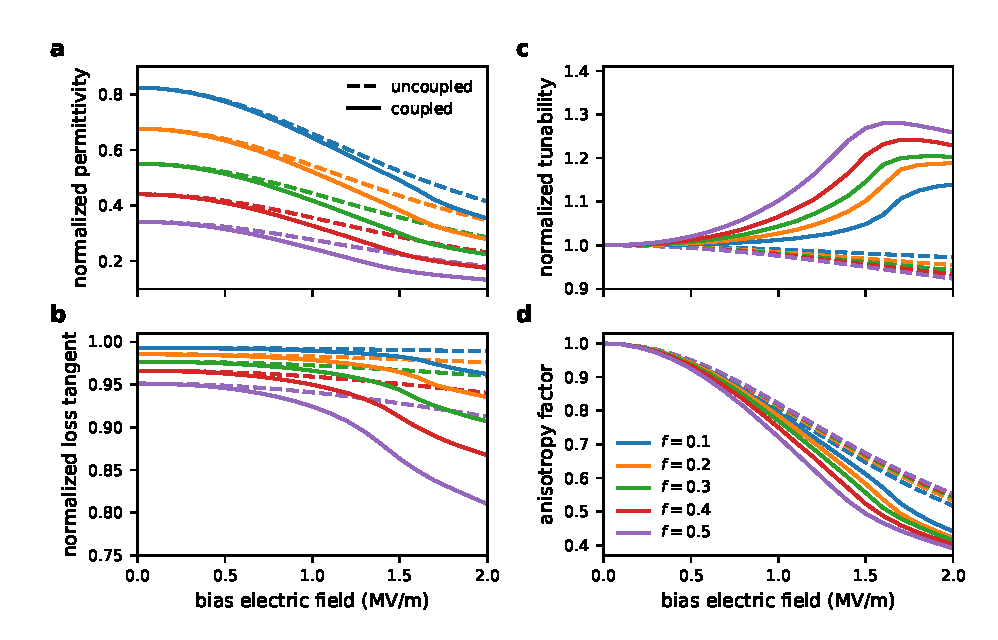
\includegraphics[width=1\textwidth]{effpar_per}
\caption{Effective parameters of the 2D metamaterials as a function of the
 applied electric field for various filling fraction of dielectric.
 (a): normalized permittivity, (b): normalized loss tangent, (c): normalized tunability and
 (d): anisotropy factor. The solid lines correspond to the coupled model and
 the dashed lines to the uncoupled model.}
\label{eff_par_2D_TM}
\end{figure}


% -------------------------------------------------------------------------------
\subsection{Random case}
\begin{figure}
\centering
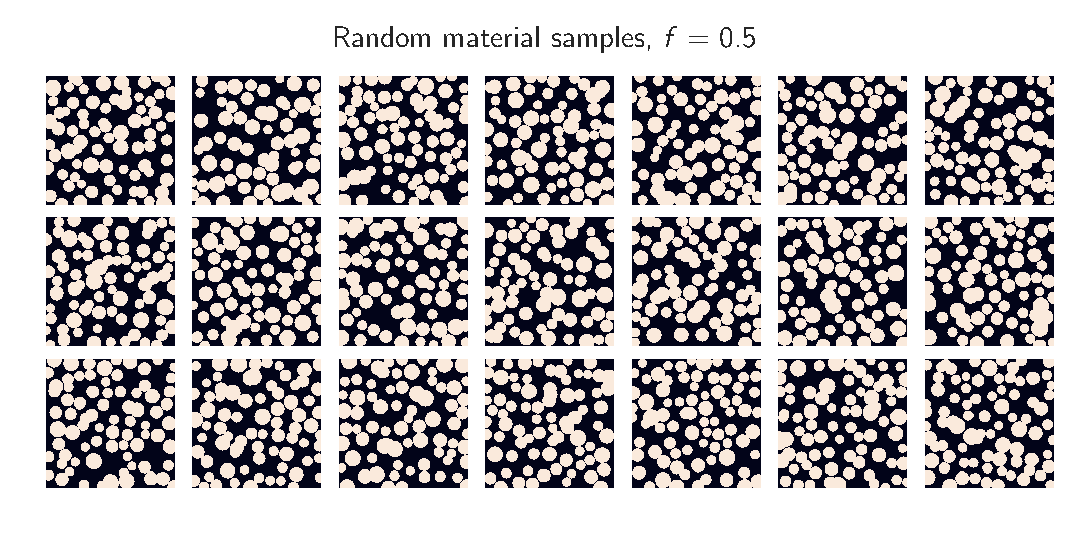
\includegraphics[width=0.8\columnwidth]{randmatepsi}
\caption{Permittivity distribution of the numerical samples used for $f=0.5$. Dark
colour indicates the ferroelectric material while light colour represents the
dielectric inclusions.}
\label{randmatepsi}
\end{figure}

We finally study the effect of random particle distribution on the effective parameters of the
composites. This is an important point as fabrication of randomly dispersed
inclusions is much more easy from a technological perspective. For each filling fraction of the dielectric,
we generated 21 numerical samples with inclusions of circular cross section of average radius
$r=d/20$ that can vary by $\pm 30\%$. Their centre is chosen randomly and the
rods are allowed to overlap. An example of distribution for $f=0.5$ is given on \fig{randmatepsi}.
The effective material properties are plotted on \fig{eff_par_2Drand_TM}.
Similarly to the periodic case, the permittivity decreases with increasing dilution of
ferroelectric, but for identical filling fraction,
the permittivity is lower as compared to the periodic array, and the smaller the dielectric concentration the larger
is the difference. Losses decrease as well and the reduction is substantially larger
than the periodic case, with higher variation from sample to sample as $f$ increases.
The tunability is reduced as one adds more dielectric, but is slightly greater than that in the periodic case.
The redistribution of electric field, permittivity and convergence of
the effective parameters are displayed in \fig{conv_random}. The effect of
disorder plays an important role here: the electrostatic field gets concentrated
in between neighbouring inclusions and the smaller the gap the higher the field, hence
a greater local permittivity change. In addition, even if the distribution of particle is
random, one expects that the anisotropy due to geometry would cancel for a sufficiently large number
of particles (which is the case as the mean anisotropy factor is close to $1$ when no
bias field is applied). However, the anisotropy due to ferroelectric properties is
important in this case as well, as both the $x$ and $y$ components of the electrostatic field
are playing a role. This result in an anisotropy factor that might be greater than $1$,
but with high variability from sample to sample. However, on average, the anisotropy factor
increases with increasing dielectric concentration, and the smaller the concentration the more tunable
it will be.





\begin{figure}[!t]
\centering
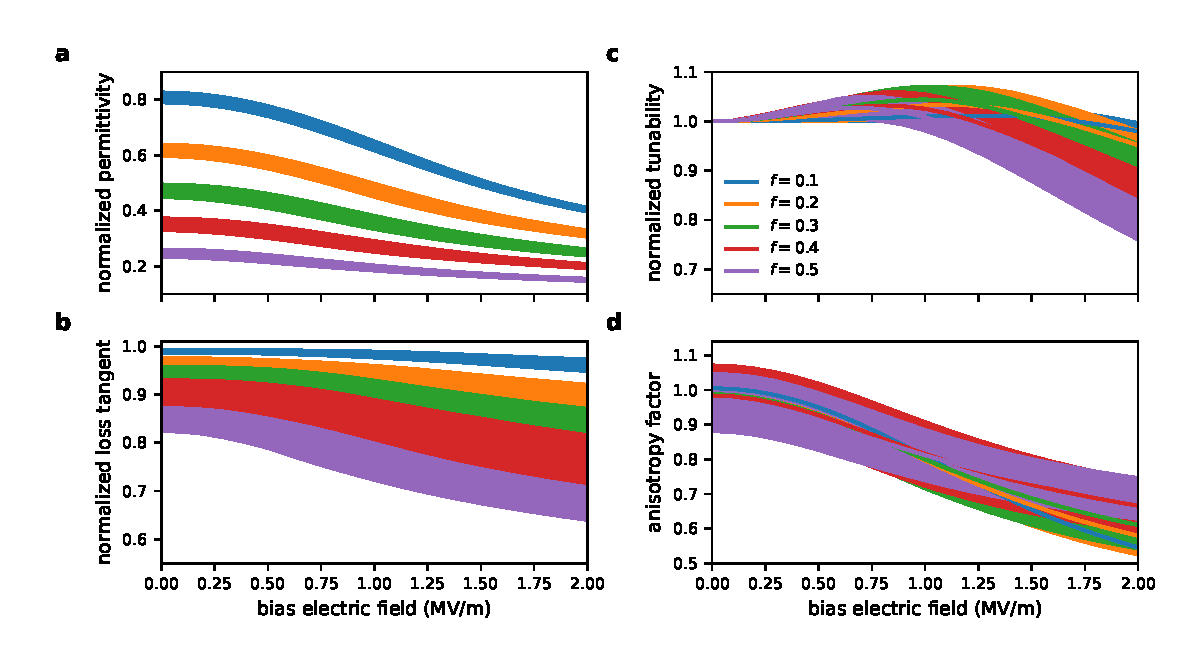
\includegraphics[width=1\textwidth]{effpar_rand_cpl}
\caption{Effective parameters of the random 2D mixtures as a function of the
 applied electric field for various filling fraction of dielectric, when the
 coupling is taken into account.
 (a): normalized permittivity, (b): normalized loss tangent, (c): normalized tunability and
 (d): anisotropy factor. The solid lines represent the average values
  over the 21 samples and the lighter error bands show a confidence interval corresponding to
  the standard deviation.}
\label{eff_par_2Drand_TM}
\end{figure}
%
%
%
\begin{figure}[!t]
\centering
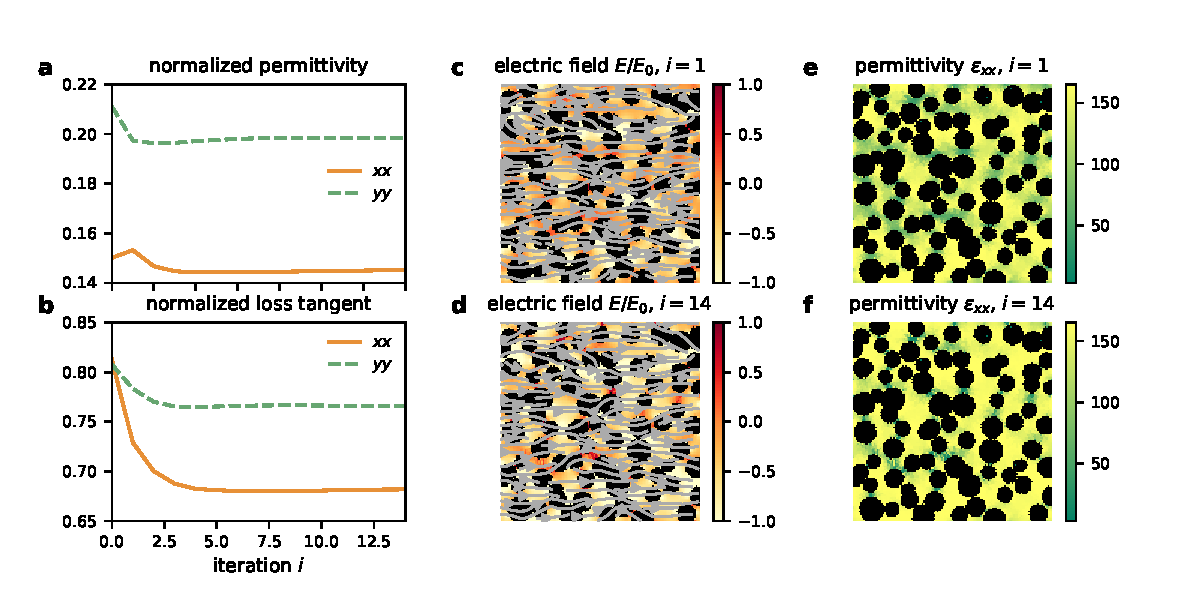
\includegraphics[width=1\textwidth]{conv_rand}
\caption{Convergence of the coupled problem in the random case
for one sample.
Real part (a) and loss tangent (b) of the components of the homogenized
 permittivity tensor as a function of iteration step $i$. The distribution of
 the normalized electric field (colour map: magnitude in logarithmic scale, arrows: direction) and of the
 $xx$ component of the permittivity tensor are shown for $i=1$
  (c and d) and $i=14$ (e and f).
 }
\label{conv_random}
\end{figure}

%#########################################################################################

\section{Conclusion}

We have studied the homogenized properties of dielectric/ferroelectric mixtures
using a rigorous model that take into account the coupling between the electrostatic
field distribution and the field dependant ferroelectric permittivity tensor. After
convergence of the coupled problem, the effective permittivity tensor is calculated using
two scale convergence homogenization theory.
The results obtained by this model differ significantly from a simple assumption that
the permittivity of the ferroelectric respond just to the uniform biasing field.
We have considered both periodic and random arrays
of dielectric rods in a ferroelectric matrix in 2D, and studied their effective properties
for TM polarization as a function of dielectric concentration and bias field.
Importantly, adding more low index and low loss dielectric allows to decrease
the overall permittivity significantly and slightly lower the losses. On the other hand,
the higher the dielectric concentration the smaller the tunability would be while
anisotropy gets higher as the concentration decreases.
The properties of the composites are affected by multiple factors:
 geometry and the spatially dependent electric field that will induce locally a tunable, anisotropic
 response in the ferroelectric phase depending on its amplitude and direction.
 This suggest that the performances of the composites
 may be enhanced by distributing the two phases in an optimal way to get high
  tunability and low losses. Further work in that direction is needed as well as
  extending this study to 3D media.
 Finally, because the permittivity of the dielectric is much smaller than the ferroelectric one,
 it would be of great interest to use high contrast homogenization theory
 \cite{bouchitte_homogenization_2004, cherednichenko_homogenization_2015} to
 study this kind of mixtures.
 This would reveal the frequency dependant artificial magnetism due to "micro-resonances"
 in the high index phase and potentially lead to composites with tunable effective permeability.



\vskip6pt

\enlargethispage{20pt}

\ethics{Insert ethics text here.}

\dataccess{Insert data accessibility text here. '(If no information, then please include the text ``This article has no additional data'').}

\aucontribute{Insert author contributions text here (to be included if more than one author).}

\competing{The authors declare no competing interrests.}

\funding{his work was funded by the Engineering and Physical Sciences Research Council (EPSRC), UK, under a grant (EP/P005578/1) 'Adaptive Tools for Electromagnetics and Materials Modelling to Bridge the Gap between Design and Manufacturing (AOTOMAT)'.}

\ack{The authors would like to thanks Henry Giddens for performing the measurements of ferroelectric permittivity used in this paper.}

\disclaimer{Insert disclaimer text here.}



%%%%%%%%%% Insert bibliography here %%%%%%%%%%%%%%

\vskip2pc

% \begin{thebibliography}{9}
%
% \end{thebibliography}

\bibliographystyle{RS}
\bibliography{biblio}

\end{document}
%
%
%
% \begin{fmtext}
% \section{Insert A head here}
% %%%% Insert A head here
%
% This demo file is intended to serve as a ``starter file''
% for rsproca journal papers produced under \LaTeX\ using
% rsproca\_new.cls v1.0.
%
% \subsection{Insert B head here}
% %%%% Insert B head here
% Subsection text here.
%
% \subsubsection{Insert C head here}
% %%%% Insert C head here
% Subsubsection text here.
%
% \section{Equations}
%
% Sample equations.
%
% %%% Numbered equation
% \begin{align}\label{1.1}
% \begin{split}
% \frac{\partial u(t,x)}{\partial t} &= Au(t,x) \left(1-\frac{u(t,x)}{K}\right)-B\frac{u(t-\tau,x) w(t,x)}{1+Eu(t-\tau,x)},\\
% \frac{\partial w(t,x)}{\partial t} &=\delta \frac{\partial^2w(t,x)}{\partial x^2}-Cw(t,x)+D\frac{u(t-\tau,x)w(t,x)}{1+Eu(t-\tau,x)},
% \end{split}
% \end{align}
%
% \begin{align}\label{1.2}
% \begin{split}
% \frac{dU}{dt} &=\alpha U(t)(\gamma -U(t))-\frac{U(t-\tau)W(t)}{1+U(t-\tau)},\\
% \frac{dW}{dt} &=-W(t)+\beta\frac{U(t-\tau)W(t)}{1+U(t-\tau)}.
% \end{split}
% \end{align}
%
% %%%% Unnumbered equation
% \begin{eqnarray}
% \frac{\partial(F_1,F_2)}{\partial(c,\omega)}_{(c_0,\omega_0)} = \left|
% \begin{array}{ll}
% \frac{\partial F_1}{\partial c} &\frac{\partial F_1}{\partial \omega} \\\noalign{\vskip3pt}
% \frac{\partial F_2}{\partial c}&\frac{\partial F_2}{\partial \omega}
% \end{array}\right|_{(c_0,\omega_0)}\notag\\
% =-4c_0q\omega_0 -4c_0\omega_0p^2 =-4c_0\omega_0(q+p^2)>0.
% \end{eqnarray}
% \end{fmtext}
%
% %%%%%%%%%%%%%%% End of first page %%%%%%%%%%%%%%%%%%%%%
%
% \maketitle
%
% \section{Enunciations}
%
% \begin{theorem}\label{T0.1}
% Assume that $\alpha>0, \gamma>1, \beta>\frac{\gamma+1}{\gamma-1}$.
% Then there exists a small $\tau_1>0$, such that for $\tau\in
% [0,\tau_1)$, if $c$ crosses $c(\tau)$ from the direction of
% to  a small amplitude periodic traveling wave solution of
% (2.1), and the period of $(\check{u}^p(s),\check{w}^p(s))$ is
% \[
% \check{T}(c)=c\cdot \left[\frac{2\pi}{\omega(\tau)}+O(c-c(\tau))\right].
% \]
% \end{theorem}
%
%
% \begin{condition}\label{C2.2}
% From (0.8) and (2.10), it holds
% $\frac{d\omega}{d\tau}<0,\frac{dc}{d\tau}<0$ for $\tau\in
% [0,\tau_1)$. This fact yields that the system (2.1) with delay
% $\tau>0$ has the periodic traveling waves for smaller wave speed $c$
% than that the system (2.1) with $\tau=0$ does. That is, the
% delay perturbation stimulates an early occurrence of the traveling waves.
% \end{condition}
%
%
% \section{Figures \& Tables}
%
% The output for figure is:\vspace*{-7pt}
%
% \begin{figure}[!h]
% %\centering\includegraphics[width=2.5in]{xxxxxx.eps}
% %%% where xxxxxx name represents "figurename.eps"
% \caption{Insert figure caption here}
% \label{fig_sim}
% \end{figure}
%
% \vspace*{-5pt}
%
% \noindent The output for table is:\vspace*{-7pt}
%
% \begin{table}[!h]
% \caption{An Example of a Table}%%%Table caption goes here
% \label{table_example}
% \begin{tabular}{llll}%%%The number of columns has to be defined here
% \hline
% date &Dutch policy &date &European policy \\
% \hline
% 1988 &Memorandum Prevention &1985 &European Directive (85/339) \\
% 1991--1997 &{\bf Packaging Covenant I} & & \\
% 1994 &Law Environmental Management &1994 &European Directive (94/62) \\
% 1997 &Agreement Packaging and Packaging Waste & & \\\hline
% \end{tabular}
% \vspace*{-4pt}
% \end{table}%%%End of the table
%
% \section{Conclusion}
% The conclusion text goes here.
%
% \vskip6pt
%
% \enlargethispage{20pt}
%
% \ethics{Insert ethics text here.}
%
% \dataccess{Insert data accessibility text here. '(If no information, then please include the text ``This article has no additional data'').}
%
% \aucontribute{Insert author contributions text here (to be included if more than one author).}
%
% \competing{Insert competing interests text here.}
%
% \funding{Insert funding text here.}
%
% \ack{Insert acknowledgment text here.}
%
% \disclaimer{Insert disclaimer text here.}
%
% %%%%%%%%%% Insert bibliography here %%%%%%%%%%%%%%
%
% \vskip2pc
%
% % \begin{thebibliography}{9}
% %
% % \end{thebibliography}
%
% \bibliographystyle{RS}
% \bibliography{biblio}
